%%%%%%%%%%%%%%%%%%%%%%%%%%%%%%%%%%%%%%%%%
% Journal Article
% LaTeX Template
% Version 1.4 (15/5/16)
%
% This template has been downloaded from:
% http://www.LaTeXTemplates.com
%
% Original author:
% Frits Wenneker (http://www.howtotex.com) with extensive modifications by
% Vel (vel@LaTeXTemplates.com)
%
% License:
% CC BY-NC-SA 3.0 (http://creativecommons.org/licenses/by-nc-sa/3.0/)
%
%%%%%%%%%%%%%%%%%%%%%%%%%%%%%%%%%%%%%%%%%

%----------------------------------------------------------------------------------------
%	PACKAGES AND OTHER DOCUMENT CONFIGURATIONS
%----------------------------------------------------------------------------------------

%\documentclass[twoside,twocolumn]{article}
\documentclass[oneside,onecolumn]{article}

\usepackage{subfigure}% Support for small, `sub' figures and tables
\usepackage{float} 
\usepackage{array}
\usepackage{graphicx}
\usepackage{amsmath}  % line in equations
\usepackage{blindtext} % Package to generate dummy text throughout this template 

\usepackage[sc]{mathpazo} % Use the Palatino font
\usepackage[T1]{fontenc} % Use 8-bit encoding that has 256 glyphs
\linespread{1.05} % Line spacing - Palatino needs more space between lines
\usepackage{microtype} % Slightly tweak font spacing for aesthetics

\usepackage[english]{babel} % Language hyphenation and typographical rules

\usepackage[hmarginratio=1:1,top=32mm,columnsep=20pt]{geometry} % Document margins
\usepackage[hang, small,labelfont=bf,up,textfont=it,up]{caption} % Custom captions under/above floats in tables or figures
\usepackage{booktabs} % Horizontal rules in tables

%\usepackage{lettrine} % The lettrine is the first enlarged letter at the beginning of the text
\usepackage{enumitem} % Customized lists
\setlist[itemize]{noitemsep} % Make itemize lists more compact

\usepackage{abstract} % Allows abstract customization
\renewcommand{\abstractnamefont}{\normalfont\bfseries} % Set the "Abstract" text to bold
\renewcommand{\abstracttextfont}{\normalfont\small\itshape} % Set the abstract itself to small italic text

\usepackage{titlesec} % Allows customization of titles
\renewcommand\thesection{\Roman{section}} % Roman numerals for the sections
\renewcommand\thesubsection{\roman{subsection}} % roman numerals for subsections
%\titleformat{\section}[block]{\large\scshape\centering}{\thesection.}{1em}{} % Change the look of the section titles
\titleformat{\section}[block]{\large\scshape}{\thesection.}{1em}{} % Change the look of the section titles
\titleformat{\subsection}[block]{\large}{\thesubsection.}{1em}{} % Change the look of the section titles

\usepackage{fancyhdr} % Headers and footers
\pagestyle{fancy} % All pages have headers and footers
\fancyhead{} % Blank out the default header
\fancyfoot{} % Blank out the default footer
%\fancyhead[C]{Running title $\bullet$ May 2016 $\bullet$ Vol. XXI, No. 1} % Custom header text
\fancyfoot[RO,LE]{\thepage} % Custom footer text

\usepackage{titling} % Customizing the title section

\usepackage{hyperref} % For hyperlinks in the PDF



\usepackage{listings} % code listing
\usepackage{color}

\definecolor{dkgreen}{rgb}{0,0.6,0}
\definecolor{gray}{rgb}{0.5,0.5,0.5}
\definecolor{mauve}{rgb}{0.58,0,0.82}

\lstset{frame=tb,
	language=Java,
	aboveskip=3mm,
	belowskip=3mm,
	showstringspaces=false,
	columns=flexible,
	basicstyle={\small\ttfamily},
	numbers=none,
	numberstyle=\tiny\color{gray},
	keywordstyle=\color{blue},
	commentstyle=\color{dkgreen},
	stringstyle=\color{mauve},
	breaklines=true,
	breakatwhitespace=true,
	tabsize=3
}
%----------------------------------------------------------------------------------------
%	TITLE SECTION
%----------------------------------------------------------------------------------------

\setlength{\droptitle}{-4\baselineskip} % Move the title up

\pretitle{\begin{center}\Huge\bfseries} % Article title formatting
\posttitle{\end{center}} % Article title closing formatting
\title{CS557: Project 3} % Article title
\author{%
\textsc{Chao Huang Lin} \\[1ex] % Your name
%\textsc{Chao Huang Lin}\thanks{A thank you or further information} \\[1ex] % Your name
\normalsize Central Washington University \\ % Your institution
\normalsize \href{mailto: chao.huanglin@cwu.edu}{chao.huanglin@cwu.edu} % Your email address
%\and % Uncomment if 2 authors are required, duplicate these 4 lines if more
%\textsc{Jane Smith}\thanks{Corresponding author} \\[1ex] % Second author's name
%\normalsize University of Utah \\ % Second author's institution
%\normalsize \href{mailto:jane@smith.com}{jane@smith.com} % Second author's email address
}
\date{\today} % Leave empty to omit a date
\renewcommand{\maketitlehookd}{%
%\begin{abstract}
%\noindent \blindtext % Dummy abstract text - replace \blindtext with your abstract text
%\end{abstract}
}

%----------------------------------------------------------------------------------------

\begin{document}

% Print the title
\maketitle

%----------------------------------------------------------------------------------------
%	ARTICLE CONTENTS
%----------------------------------------------------------------------------------------
Maximize the function using genetic algorithm, write your own code. Use the following operators: Selection, Crossover, and Mutation.



\begin{equation}
f(x,y) = sin(\pi*10*x+10/(1+y^2)) + ln(x^2+y^2), 3 \leq x \leq 10, 4 \leq y \leq 8
\end{equation}




The plot of the function with python matplotlib is shown in the figure \ref{fig:function}.


\section{implementation}

The Genetic Algorithm (GA) code was implemented in python, the basic structure of the ga is based on an array of unsigned integer 32 where 16 bits are assigned for x values and the other 16 bits are assigned to y values.
All the operation of Selection, Crossover, Mutation, and Elitism was developed with binary operators  ( \& | >> << \(\sim\))   which modify directly on the bit value.
The conversion of x and y values in 16 bits unsigned integer format to real number representation  is described in the following formulas:

\begin{equation}
\begin{split}
x_{real} = 3 + x_{uint} * 7/(2^{16} -1) \\
y_{real} = 4 + y_{unit} * 4/(2^{16} -1)
\end{split}
\end{equation}

where \( x_{real}\) and \(y_{real}\) are real number representation of x and y respectively, \( x_{uint}\) and \(y_{uint}\)   are unsigned int representation of x and y respectively.

\section{Result}

\subsection{Comparing the result with mutation probability of 0.0003125}


For this result, we used a population of 1000, the number of generations was set to 50, and the mutation probability was 0.0003125.

The figure \ref{fig:lowmutation} display the evolution of  Maximum f(x,y) and the Average f(x,y) of three type of Genetic Algorithm, these are: 
\begin{itemize}
\item \textbf{Selection + Crossover}: The selection process is based on fitness probability, for crossover two strings are selected, and then the string are combined randomly to create two children in the new population. 
\item \textbf{Selection + Crossover + Mutation}: After selection and crossover, the mutation is apllied which changes the bit of the string when the probability of mutation of the certain bit is lower than the mutation probability threshold.
\item \textbf{Selection + Crossover + Mutation + Elitism}: The elitism used in this project selects the best 5\% strings of the old population and replace the worse  5\% of the new population.

\end{itemize}



the maximum value of f(x, y) and the values of x and y for which this maximum is obtained of each type of GA is described in listing \ref{list:lowmutation}
\begin{figure}[H]
	\centering

	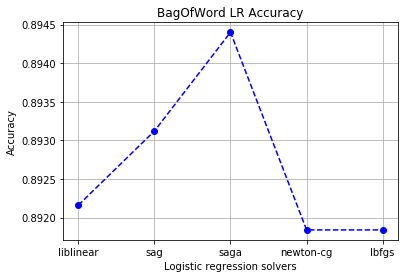
\includegraphics[height=5cm]{report_plot/plot_bagofword/logistic_regression_accuracy.png}
	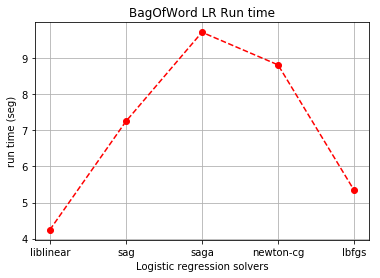
\includegraphics[height=5cm]{report_plot/plot_bagofword/logistic_regression_runtime.png}
	
	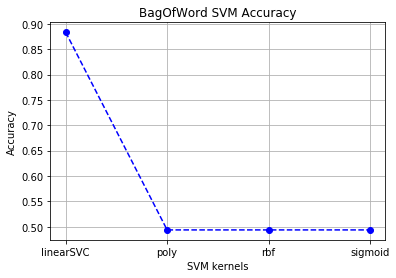
\includegraphics[height=5cm]{report_plot/plot_bagofword/svm_accuracy.png}
	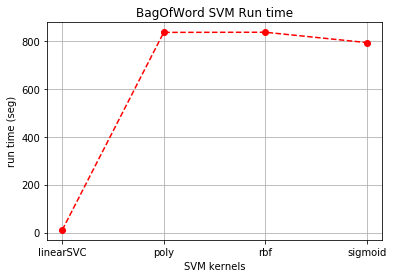
\includegraphics[height=5cm]{report_plot/plot_bagofword/svm_runtime.png}
	
	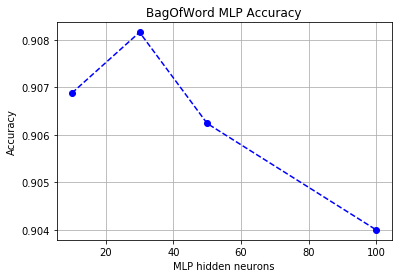
\includegraphics[height=5cm]{report_plot/plot_bagofword/mlp_accuracy.png}
	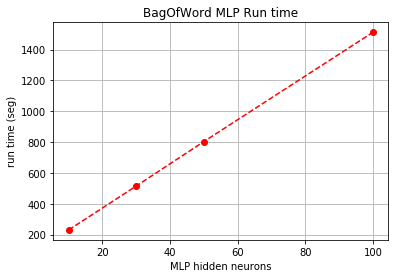
\includegraphics[height=5cm]{report_plot/plot_bagofword/mlp_runtime.png}
	
	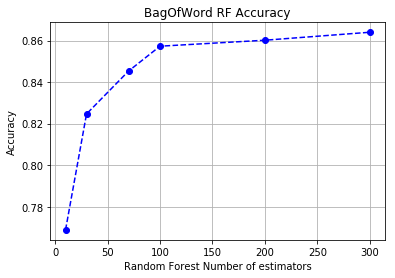
\includegraphics[height=5cm]{report_plot/plot_bagofword/rf_accuracy.png}
	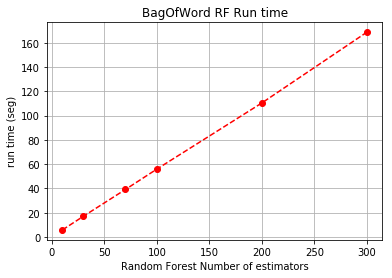
\includegraphics[height=5cm]{report_plot/plot_bagofword/rf_runtime.png}



	%\includegraphics[width=0.40\linewidth]{figures/Train2result.png}
	\caption{Bag of word and different algorithms for classification} 
	\label{fig:lowmutation}
\end{figure}

\begin{lstlisting}[language=Python, caption={Using Mutation probability = 0.0003125}, label={list:lowmutation}]

Time passed: 0.0hour:0.0min:25.433627367019653sec
Reviews Matrix Shape (25000, 150000)
----------
####### Logistic Regression #######
Accuracy for Logistic Regression liblinear: 0.89216
[[2718  367]
[ 307 2858]]
Time passed: 0.0hour:0.0min:4.241924524307251sec
----------
Accuracy for Logistic Regression sag: 0.89312
[[2721  364]
[ 304 2861]]
Time passed: 0.0hour:0.0min:7.24403715133667sec
----------
Accuracy for Logistic Regression saga: 0.8944
[[2729  356]
[ 304 2861]]
Time passed: 0.0hour:0.0min:9.71173644065857sec
----------
Accuracy for Logistic Regression newton-cg: 0.89184
[[2717  368]
[ 308 2857]]
Time passed: 0.0hour:0.0min:8.808095932006836sec
----------
Accuracy for Logistic Regression lbfgs: 0.89184
[[2717  368]
[ 308 2857]]
Time passed: 0.0hour:0.0min:5.3367016315460205sec
----------
####### SVM #######
Accuracy for SVM linearSVC: 0.88352
[[2694  391]
[ 337 2828]]
Time passed: 0.0hour:0.0min:10.819516658782959sec
----------
Accuracy for SVM poly: 0.4936
[[3085    0]
[3165    0]]
Time passed: 0.0hour:13.0min:56.243077993392944sec
----------
Accuracy for SVM rbf: 0.4936
[[3085    0]
[3165    0]]
Time passed: 0.0hour:13.0min:56.82241249084473sec
----------
Accuracy for SVM sigmoid: 0.4936
[[3085    0]
[3165    0]]
Time passed: 0.0hour:13.0min:13.656466484069824sec
----------
####### MLP #######
Accuracy for MLP hidden neurons 10: 0.90688
[[2765  320]
[ 262 2903]]
Time passed: 0.0hour:3.0min:50.4915292263031sec
----------
Accuracy for MLP hidden neurons 30: 0.90816
[[2763  322]
[ 252 2913]]
Time passed: 0.0hour:8.0min:35.47192716598511sec
----------
Accuracy for MLP hidden neurons 50: 0.90624
[[2761  324]
[ 262 2903]]
Time passed: 0.0hour:13.0min:23.848541259765625sec
----------
Accuracy for MLP hidden neurons 100: 0.904
[[2757  328]
[ 272 2893]]
Time passed: 0.0hour:25.0min:12.753307104110718sec
----------
####### Random Forest #######
Accuracy for Random Forest, n estimators 10: 0.7688
[[2569  516]
[ 929 2236]]
Time passed: 0.0hour:0.0min:5.870083570480347sec
----------
Accuracy for Random Forest, n estimators 30: 0.82464
[[2589  496]
[ 600 2565]]
Time passed: 0.0hour:0.0min:17.115859031677246sec
----------
Accuracy for Random Forest, n estimators 70: 0.84528
[[2624  461]
[ 506 2659]]
Time passed: 0.0hour:0.0min:39.14116311073303sec
----------
Accuracy for Random Forest, n estimators 100: 0.85728
[[2644  441]
[ 451 2714]]
Time passed: 0.0hour:0.0min:55.942787408828735sec
----------
Accuracy for Random Forest, n estimators 200: 0.86016
[[2629  456]
[ 418 2747]]
Time passed: 0.0hour:1.0min:50.35554027557373sec
----------
Accuracy for Random Forest, n estimators 300: 0.864
[[2641  444]
[ 406 2759]]
Time passed: 0.0hour:2.0min:48.58206343650818sec
----------

\end{lstlisting}

\begin{figure}[H]
	\centering
	
	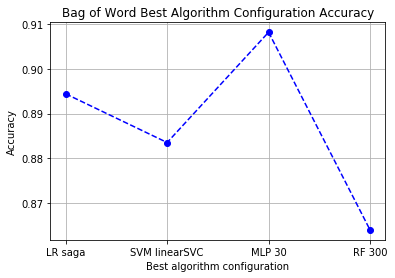
\includegraphics[height=5cm]{report_plot/plot_bagofword/best_accuracy.png}
	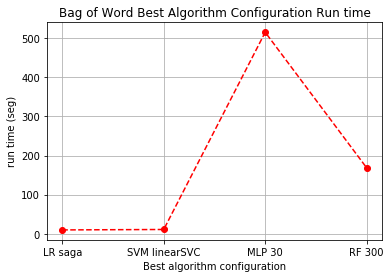
\includegraphics[height=5cm]{report_plot/plot_bagofword/best_alg_runtime.png}

	%\includegraphics[width=0.40\linewidth]{figures/Train2result.png}
	\caption{Best algorithm for bag of word} 
	\label{fig:lowmutation}
\end{figure}


\begin{figure}[H]
	\centering
	
	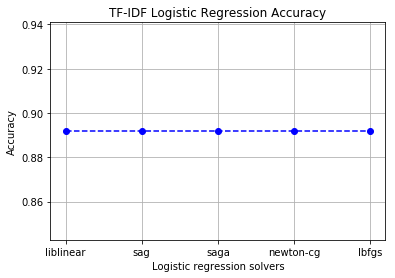
\includegraphics[height=5cm]{report_plot/plot_tfidf/logistic_regression_accuracy.png}
	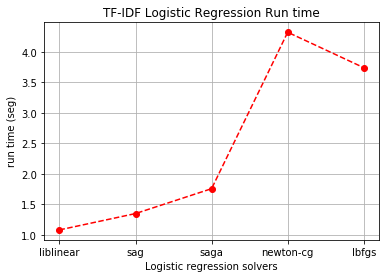
\includegraphics[height=5cm]{report_plot/plot_tfidf/logistic_regression_runtime.png}
	
	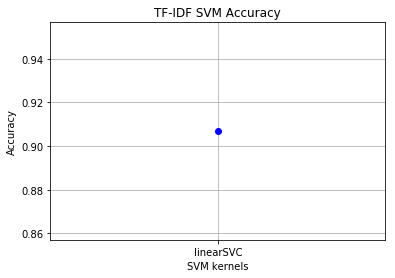
\includegraphics[height=5cm]{report_plot/plot_tfidf/svm_accuracy.png}
	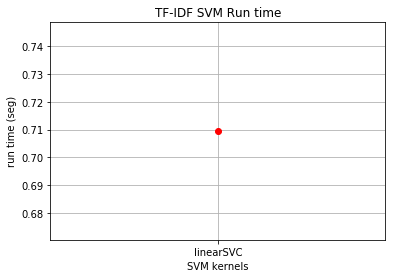
\includegraphics[height=5cm]{report_plot/plot_tfidf/svm_runtime.png}
	
	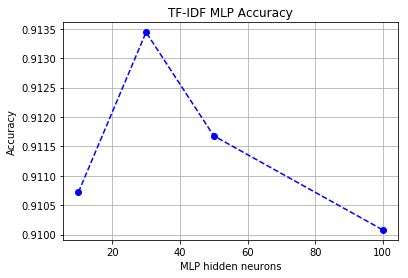
\includegraphics[height=5cm]{report_plot/plot_tfidf/mlp_accuracy.png}
	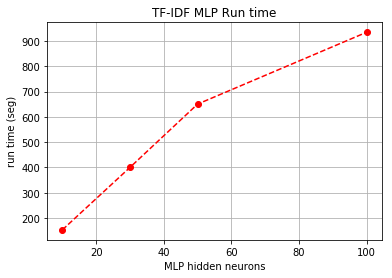
\includegraphics[height=5cm]{report_plot/plot_tfidf/mlp_runtime.png}
	
	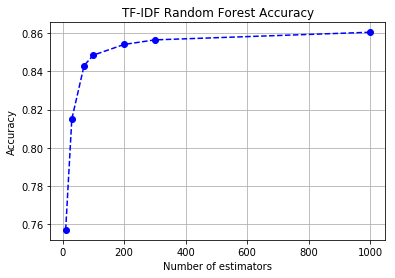
\includegraphics[height=5cm]{report_plot/plot_tfidf/rf_accuracy.png}
	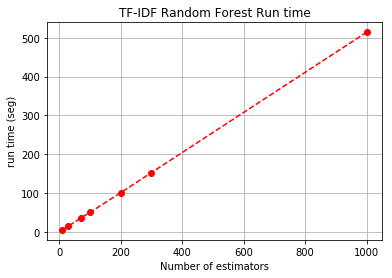
\includegraphics[height=5cm]{report_plot/plot_tfidf/rf_runtime.png}
	
	
	
	%\includegraphics[width=0.40\linewidth]{figures/Train2result.png}
	\caption{TF-IDF and different algorithms for classification} 
	\label{fig:lowmutation}
\end{figure}

\begin{lstlisting}[language=Python, caption={Using Mutation probability = 0.03}, label={list:highmutation}]

--------------max_features=150000---------------------------
Time passed: 0.0hour:0.0min:25.176562786102295sec
Reviews Matrix Shape (25000, 150000)
----------
####### Logistic Regresion #######
Accuracy for Logistic Regression liblinear: 0.89184
[[2754  356]
[ 320 2820]]
Time passed: 0.0hour:0.0min:1.0797488689422607sec
----------
Accuracy for Logistic Regression sag: 0.89184
[[2754  356]
[ 320 2820]]
Time passed: 0.0hour:0.0min:1.347956895828247sec
----------
Accuracy for Logistic Regression saga: 0.89184
[[2754  356]
[ 320 2820]]
Time passed: 0.0hour:0.0min:1.7561957836151123sec
----------
Accuracy for Logistic Regression newton-cg: 0.89184
[[2754  356]
[ 320 2820]]
Time passed: 0.0hour:0.0min:4.32199764251709sec
----------
Accuracy for Logistic Regression lbfgs: 0.89184
[[2754  356]
[ 320 2820]]
Time passed: 0.0hour:0.0min:3.7405946254730225sec
----------
####### SVM #######
Accuracy for SVM linearSVC: 0.90688
[[2818  292]
[ 290 2850]]
Time passed: 0.0hour:0.0min:0.7094793319702148sec
----------
####### MLP #######
Accuracy for MLP hidden neurons 10: 0.91072
[[2843  267]
[ 291 2849]]
Time passed: 0.0hour:2.0min:32.980093002319336sec
----------
Accuracy for MLP hidden neurons 30: 0.91344
[[2825  285]
[ 256 2884]]
Time passed: 0.0hour:6.0min:40.0584762096405sec
----------
Accuracy for MLP hidden neurons 50: 0.91168
[[2833  277]
[ 275 2865]]
Time passed: 0.0hour:10.0min:50.59632396697998sec
----------
Accuracy for MLP hidden neurons 100: 0.91008
[[2852  258]
[ 304 2836]]
Time passed: 0.0hour:15.0min:34.89562630653381sec
----------
####### Random Forest #######
Accuracy for Random Forest, n estimators 10: 0.75696
[[2608  502]
[1017 2123]]
Time passed: 0.0hour:0.0min:5.341684103012085sec
----------
Accuracy for Random Forest, n estimators 30: 0.81504
[[2625  485]
[ 671 2469]]
Time passed: 0.0hour:0.0min:15.463613033294678sec
----------
Accuracy for Random Forest, n estimators 70: 0.84304
[[2665  445]
[ 536 2604]]
Time passed: 0.0hour:0.0min:35.642505407333374sec
----------
Accuracy for Random Forest, n estimators 100: 0.84848
[[2666  444]
[ 503 2637]]
Time passed: 0.0hour:0.0min:50.5357141494751sec
----------
Accuracy for Random Forest, n estimators 200: 0.85408
[[2665  445]
[ 467 2673]]
Time passed: 0.0hour:1.0min:41.000643491744995sec
----------
Accuracy for Random Forest, n estimators 300: 0.85648
[[2663  447]
[ 450 2690]]
Time passed: 0.0hour:2.0min:32.89604187011719sec
----------
Accuracy for Random Forest, n estimators 1000: 0.86048
[[2672  438]
[ 434 2706]]
Time passed: 0.0hour:8.0min:34.136587381362915sec
----------

\end{lstlisting}


\begin{figure}[H]
	\centering
	
	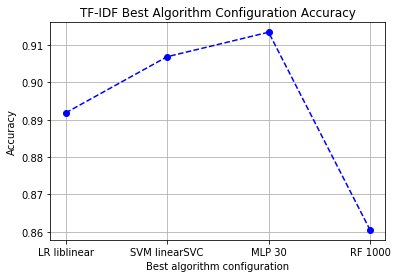
\includegraphics[height=5cm]{report_plot/plot_tfidf/best_accuracy.png}
	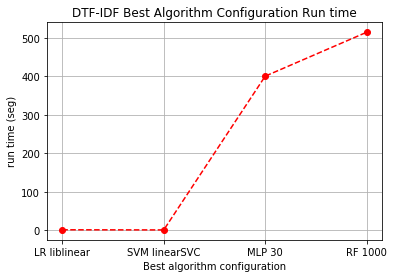
\includegraphics[height=5cm]{report_plot/plot_tfidf/best_alg_runtime.png}
	
	%\includegraphics[width=0.40\linewidth]{figures/Train2result.png}
	\caption{Best algorithm for TF-IDF} 
	\label{fig:lowmutation}
\end{figure}



\begin{figure}[H]
	\centering
	
	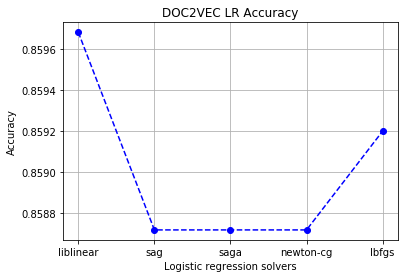
\includegraphics[height=5cm]{report_plot/plot_doc2vec/logistic_regression_accuracy.png}
	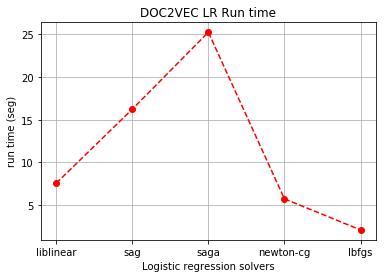
\includegraphics[height=5cm]{report_plot/plot_doc2vec/logistic_regression_runtime.png}
	
	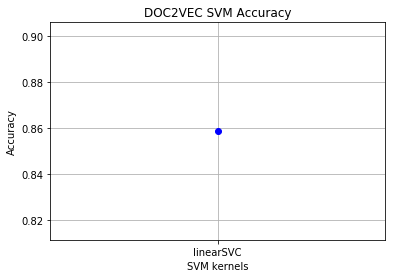
\includegraphics[height=5cm]{report_plot/plot_doc2vec/svm_accuracy.png}
	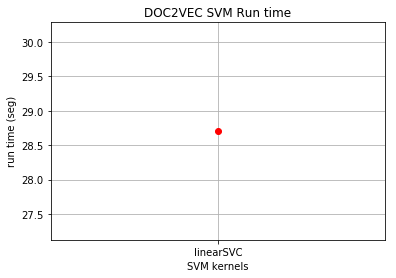
\includegraphics[height=5cm]{report_plot/plot_doc2vec/svm_runtime.png}
	
	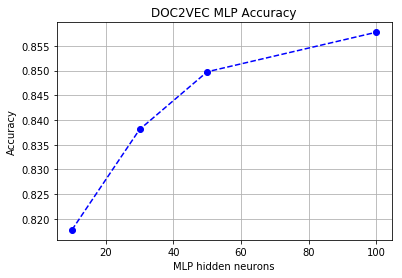
\includegraphics[height=5cm]{report_plot/plot_doc2vec/mlp_accuracy.png}
	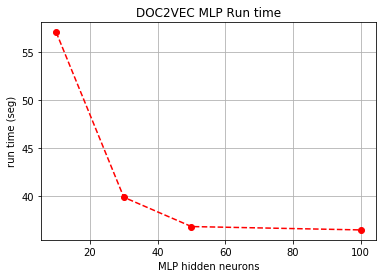
\includegraphics[height=5cm]{report_plot/plot_doc2vec/mlp_runtime.png}
	
	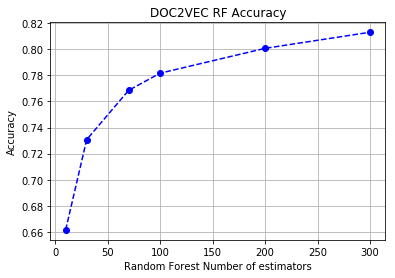
\includegraphics[height=5cm]{report_plot/plot_doc2vec/rf_accuracy.png}
	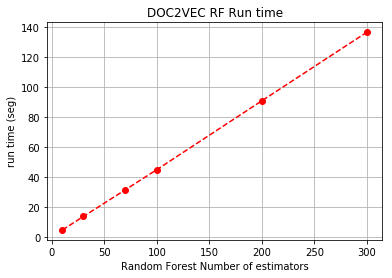
\includegraphics[height=5cm]{report_plot/plot_doc2vec/rf_runtime.png}
	
	
	
	%\includegraphics[width=0.40\linewidth]{figures/Train2result.png}
	\caption{Mutation probability =0.0003125} 
	\label{fig:lowmutation}
\end{figure}

\begin{figure}[H]
	\centering
	
	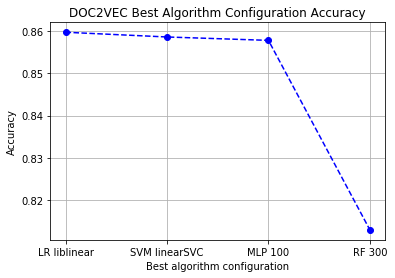
\includegraphics[height=5cm]{report_plot/plot_doc2vec/best_accuracy.png}
	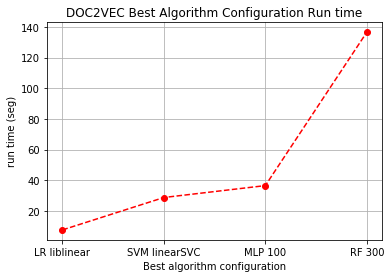
\includegraphics[height=5cm]{report_plot/plot_doc2vec/best_alg_runtime.png}
	
	%\includegraphics[width=0.40\linewidth]{figures/Train2result.png}
	\caption{Best algorith for DOC2VEC} 
	\label{fig:lowmutation}
\end{figure}


\begin{lstlisting}[language=Python, caption={Using Mutation probability = 0.03}, label={list:highmutation}]
-----vector_size=1000-------------------
Time passed: 0.0hour:9.0min:26.276705503463745sec
Reviews Matrix Shape 25000
----------
####### Logistic Regression #######
Accuracy for Logistic Regression liblinear: 0.85968
[[2690  455]
[ 422 2683]]
Time passed: 0.0hour:0.0min:7.546234130859375sec
----------
Accuracy for Logistic Regression sag: 0.85872
[[2686  459]
[ 424 2681]]
Time passed: 0.0hour:0.0min:16.22825574874878sec
----------
Accuracy for Logistic Regression saga: 0.85872
[[2686  459]
[ 424 2681]]
Time passed: 0.0hour:0.0min:25.2565176486969sec
----------
Accuracy for Logistic Regression newton-cg: 0.85872
[[2686  459]
[ 424 2681]]
Time passed: 0.0hour:0.0min:5.716395378112793sec
----------
Accuracy for Logistic Regression lbfgs: 0.8592
[[2687  458]
[ 422 2683]]
Time passed: 0.0hour:0.0min:2.0744385719299316sec
----------
####### SVM #######
Accuracy for SVM linearSVC: 0.85856
[[2684  461]
[ 423 2682]]
Time passed: 0.0hour:0.0min:28.703908681869507sec
----------
####### MLP #######
Accuracy for MLP hidden neurons 10: 0.81776
[[2573  572]
[ 567 2538]]
Time passed: 0.0hour:0.0min:57.02952313423157sec
----------
Accuracy for MLP hidden neurons 30: 0.83808
[[2625  520]
[ 492 2613]]
Time passed: 0.0hour:0.0min:39.87165451049805sec
----------
Accuracy for MLP hidden neurons 50: 0.84976
[[2662  483]
[ 456 2649]]
Time passed: 0.0hour:0.0min:36.823540449142456sec
----------
Accuracy for MLP hidden neurons 100: 0.85776
[[2673  472]
[ 417 2688]]
Time passed: 0.0hour:0.0min:36.47429847717285sec
----------
####### Random Forest #######
Accuracy for Random Forest, n estimators 10: 0.6616
[[2399  746]
[1369 1736]]
Time passed: 0.0hour:0.0min:4.635227203369141sec
----------
Accuracy for Random Forest, n estimators 30: 0.73072
[[2433  712]
[ 971 2134]]
Time passed: 0.0hour:0.0min:13.59542965888977sec
----------
Accuracy for Random Forest, n estimators 70: 0.76848
[[2466  679]
[ 768 2337]]
Time passed: 0.0hour:0.0min:31.472816705703735sec
----------
Accuracy for Random Forest, n estimators 100: 0.7816
[[2478  667]
[ 698 2407]]
Time passed: 0.0hour:0.0min:44.89513874053955sec
----------
Accuracy for Random Forest, n estimators 200: 0.80064
[[2501  644]
[ 602 2503]]
Time passed: 0.0hour:1.0min:30.825007915496826sec
----------
Accuracy for Random Forest, n estimators 300: 0.81296
[[2545  600]
[ 569 2536]]
Time passed: 0.0hour:2.0min:16.589736938476562sec
----------

\end{lstlisting}




\begin{figure}[H]
	\centering
	
	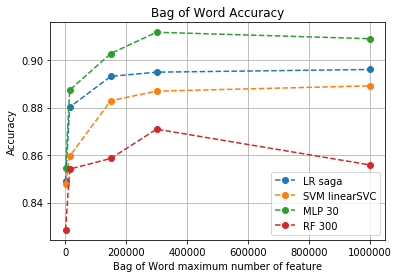
\includegraphics[height=5cm]{report_plot/plot_variable_dimension_desktop/bagofword_accurary_dimension.png}
	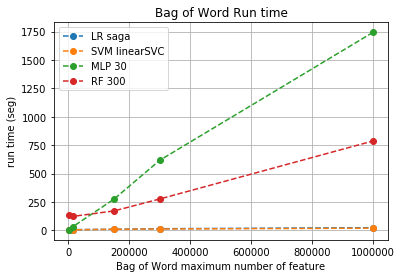
\includegraphics[height=5cm]{report_plot/plot_variable_dimension_desktop/bagofword_accurary_runtime.png}
	
	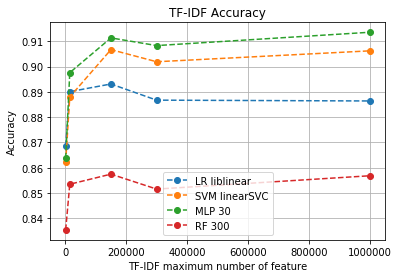
\includegraphics[height=5cm]{report_plot/plot_variable_dimension_surface/tf-idf_accurary_dimension.png}
	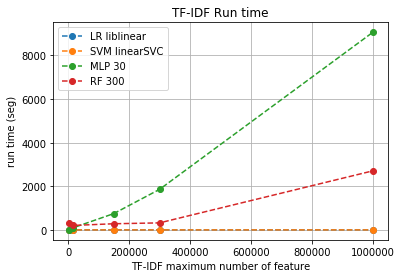
\includegraphics[height=5cm]{report_plot/plot_variable_dimension_surface/tf-idf_accurary_runtime.png}
	
	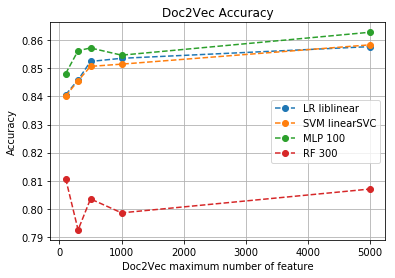
\includegraphics[height=5cm]{report_plot/plot_variable_dimension_desktop/doc2vec_accurary_dimension.png}
	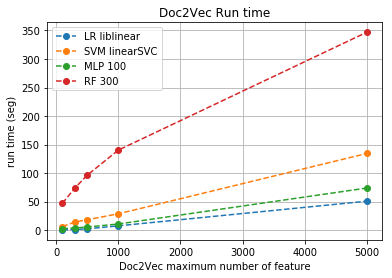
\includegraphics[height=5cm]{report_plot/plot_variable_dimension_desktop/doc2vec_accurary_runtime.png}
	

	
	
	%\includegraphics[width=0.40\linewidth]{figures/Train2result.png}
	\caption{Accuracy and processing time with different feature dimension} 
	\label{fig:lowmutation}
\end{figure}


\subsection{Comparing the result with mutation probability of 0.03}


For this result, we used a population of 1000, the number of generations was set to 50, and the mutation probability was 0.03.

The figure \ref{fig:highmutation} display the evolution of  Maximum f(x,y) and the Average f(x,y) of three type of Genetic Algorithm.

the maximum value of f(x, y) and the values of x and y for which this maximum is obtained of each type of GA is described in listing \ref{list:highmutation}






\subsection{Comparing the result with different population's size}

The result of the evolution of Maximum and Average value with different population is shown in the figures \ref{fig:low_mut_pop} and \ref{fig:high_mut_pop}. The figure \ref{fig:low_mut_pop} is obtained by using the mutation probability of 0.0003125 and the figure \ref{fig:high_mut_pop} is obtained by using the mutation probability of 0.03.



\section{Conclusion}

Many types of Genetic Algorithm have been tested in this project, all of them was able to converge and get the maximum f(x,y) close to 6.08. Despite this, the GA with (Selection + Crossover + Mutation + Elitism) performs much better than others because it keeps the best strings through all the generations. If we don't kee best string from the previous generation to the next generation, the maximum value of the population of the next generation could get worse as displayed in the figures 2 to 5, where the evolution of the maximum values of GA versions without elitism go up and down through the generations (iterations).

In addition, comparing the figures \ref{fig:lowmutation} and \ref{fig:highmutation}  when the mutation probability is too big the evolution of the maximum f(x,y) values of the  GA with (Selection + Crossover + Mutation) becomes unstable. 

Furthermore, from figures \ref{fig:low_mut_pop} and \ref{fig:high_mut_pop} we can observe when the population increase it will need less generation to converge and get the maximum value.

%------------------------------------------------


%\begin{table}
%\caption{Example table}
%\centering
%\begin{tabular}{llr}
%\toprule
%\multicolumn{2}{c}{Name} \\
%\cmidrule(r){1-2}
%First name & Last Name & Grade \\
%\midrule
%John & Doe & $7.5$ \\
%Richard & Miles & $2$ \\
%\bottomrule
%\end{tabular}
%\end{table}




%------------------------------------------------



%----------------------------------------------------------------------------------------
%	REFERENCE LIST
%----------------------------------------------------------------------------------------

%\begin{thebibliography}{99} % Bibliography - this is intentionally simple in this template

%\bibitem[Figueredo and Wolf, 2009]{Figueredo:2009dg}
%Figueredo, A.~J. and Wolf, P. S.~A. (2009).
%\newblock Assortative pairing and life history strategy - a cross-cultural
%  study.
%\newblock {\em Human Nature}, 20:317--330.
 
%\end{thebibliography}

%----------------------------------------------------------------------------------------

\end{document}
